% typeset: Pdftex
% Afterwards compile with pdflatex > bibtex > pdflatex > pdflatex
% TeXShop Settings... > Engine > BibTex Engine > biber
% beamer likes biber
% latex likes bibtex

% https://tex.stackexchange.com/questions/270633/beamer-and-the-pause-command
% https://tex.stackexchange.com/questions/1423/is-there-a-nice-way-to-compile-a-beamer-presentation-without-the-pauses
% Beamer presentation template for redux-pdes
% \documentclass[ handout ]{beamer} % for printing
\documentclass[ ]{beamer}

% Fetch home directory: make this file independent of file system
\usepackage{catchfile}
\CatchFileDef{\HomePath}{|kpsewhich -var-value=HOME}{}
% Define base paths
% relies on symlink  at /Users/dantopa/, e.g.
% 	GitHub -> /Users/dantopa//repos-xiuhcoatl/github
\makeatletter
\edef\HomePath{\expandafter\zap@space\HomePath \@empty}
\makeatother
\newcommand{\pGithub}          			{\HomePath/GitHub/}
	\newcommand{\pGithubSharing}	{\pGithub/sharing/}
	\newcommand{\pGlobal}			{\pGithubSharing/global/}
	\newcommand{\pGlobalSetup}		{\pGlobal/setup-global/}
	\newcommand{\pWorkspace}		{\pGithubSharing/beamer/redux-pdes}

% ===========================================================
% Global and Local Resource Setup
% The following lines load various global and local resource
% configurations, paths, and package lists required for the 
% document. These files are part of the shared library located
% in "~/GitHub/sharing/global/setup-global".
% ===========================================================

% Load Global Setup Files
% \input{\pGlobalSetup setup-global-beamer}

\input{\pGlobalSetup aesthetics-global.tex}
%\input{\pGlobalSetup beamer-beautify-hii.tex}
\input{\pGlobalSetup beautify-hii.tex}

\input{\pGlobalSetup paths-global.tex}
\input{\pGlobalSetup packages-global-beamer.tex}
\input{\pGlobalSetup math-global-beamer.tex}
\input{\pGlobalSetup hyperlinks-global.tex}
\input{\pGlobalSetup paths-bitbucket.tex}
\input{\pGlobalSetup libraries-global.tex}
\input{\pGlobalSetup macros-global.tex}

\input{\pGlobalSetup paths-local}

\endinput  %  -  -  -  -  -  -  -  -  -  -  -  -  -  -  -  -  -  -  -  -


% Excursion Setup Files
% \input{\pLocalSetup setup-local}

%\input{\pLocalSetup paths-local}
%\input{\pLocalSetup bibliography-local}
\input{\pLocalSetup hyperlinks-local}
%\input{\pLocalSetup input-libraries-local}

\input{\pLocalSetup macros-local}
% LaTeX macros to present a programming environment
% Looks like a terminal session, colored text on black background
\newcommand{\scru}[1]		{\bl   {\texttt{#1}}}
\newcommand{\scrk}[1]		{\bk   {\texttt{#1}}}
\newcommand{\scrg}[1]		{\gr   {\texttt{#1}}}
\newcommand{\scrr}[1]		{\rd   {\texttt{#1}}}
\newcommand{\scrv}[1]		{\dg   {\texttt{#1}}}
\newcommand{\scrz}[1]		{\mg   {\texttt{#1}}}
\newcommand{\scrc}[1]		{\textcolor{cyan}  {\texttt{#1}}}
\newcommand{\scrp}[1]		{\textcolor{purple}{\texttt{#1}}}
\newcommand{\scry}[1]		{\textcolor{yellow}{\texttt{#1}}}
\newcommand{\scrw}[1]		{\textcolor{white} {\texttt{#1}}}

%
\newcommand{\mySize}[1]		{{\normalsize{#1}}}
\newcommand{\myCanvas}[1]		{{\setbeamercolor{background canvas}{bg=black}{#1}}}
\newcommand{\myRasa}[1]		{\myCanvas{\mySize{#1}}}
\newcommand{\myFrame}[2]		{\myRasa{\begin{frame} \frametitle{#1} #2 \end{frame}}}
\newcommand{\myFoo}[2]			{\myFrame{#1}  \program \ \\[10pt] #2 \eprogram}


% tabs
%\newcommand{\tab}[0]     {\phantom{mm}}
\newcommand{\tab}[0]		{\ \ }
\newcommand{\spacer}[0]		{\ps\text{::}\ps}
\newcommand{\ps}[0]		{\phantom{m}}

% is equal?
\newcommand{\iseq}[0]		{ \overset{?}{=} }


\endinput  %  ==  ==  ==  ==  ==  ==  ==  ==  ==

% https://engineering.purdue.edu/ECN/Support/KB/Docs/LaTeXChangingTheFont
% \tiny
% \scriptsize
% \footnotesize
% \small
% \normalsize
% \large
% \Large
% \LARGE
% \huge
% \Huge% programming enviro

\endinput  %  ==  ==  ==  ==  ==  ==  ==  ==  ==


%   --   --   --   --   --   --   --   --   --   -- Bibliography
\input{\pGlobalSetup bib-config-a.tex}
%\addbibresource{\pShareBibliographies/pdes-1.bib}
\addbibresource{\pShareBibliographies/test.bib}

%   --   --   --   --   --   --   --   --   --   -- Title, Author
\title[\pdes]{\pdes:\\A Pedestrian View}
\author[Daniel Topa]{\TopaHII \\ \TopaHIIEmail}
\institute{\missiontech} 
\date{\today}

%   --   --   --   --   --   --   --   --   --   -- Structure
\begin{document}

\begin{frame}
    \titlepage
\end{frame}

\begin{frame}[ allowframebreaks ]\frametitle{Outline}
	\tableofcontents[ hideallsubsections ]
Test citation: \cite{10.5555/889797}
\end{frame}

% Main content
	% \input{\pSections/"sec-case.tex"}

\section{PDES: Why}
%
\begin{frame}\frametitle{Relevance for SDA}
\begin{enumerate}
	\item Define \pdes
	\item Space domain application
	\item Parallelism challenges and opportunities
\end{enumerate}
\end{frame}

%     %     %     %     %     %     %     %     %
\subsection{PDES Fundamentals}
\begin{frame}\frametitle{Approaches}
	I am slide
\end{frame}

%     %     %     %     %     %     %     %     %
\subsection{Literature Survey}

\begin{frame}\frametitle{\href{https://www.cs.wm.edu/~andreas/}{\bl{Stathopoulos}}: \href{https://www.cs.wm.edu/~andreas/umsa/lectures/cs-sim-pdes.pdf}{Personal Web Page} \quad \mg{\scriptsize \raisebox{0.5ex}{\cite{Stathopoulos} \ \faUnlock}}}
\center
    % Hyperlink wraps around the image for clickable access
    \href{https://www.cs.wm.edu/~andreas/umsa/lectures/cs-sim-pdes.pdf}{
    \begin{overpic}[scale=0.325]
        % Main image (splash page or graphic)
        {\pLocalGraphics tombstones/Stathopoulos}
        % Add the unlocked symbol near the bottom-right of the image
        %\put(90,5){\faUnlock}
    \end{overpic}}
\end{frame}
%
\begin{frame}\frametitle{\href{https://www.cs.cmu.edu/~bryant/pubdir/MIT-LCS-TR-188.pdf}{\bl{Bryant}}: \href{https://publications.csail.mit.edu/lcs/pubs/pdf/MIT-LCS-TR-188.pdf}{Simulation of Packet Communication Architecture Systems} \quad \mg{\scriptsize \raisebox{0.5ex}{\cite{10.5555/889797} \ \faUnlock}}}
\center
	\href{https://apps.dtic.mil/sti/pdfs/ADA048290.pdf}{
	\begin{overpic}[ scale = 0.05 ]
		{\pLocalGraphics tombstones/pdes-alpha}
	\end{overpic}}
\end{frame}
%
\begin{frame}\frametitle{\bl{Chandy} \& \href{https://www.cs.utexas.edu/~misra/scannedPdf.dir/DistrSimulation.pdf}{\bl{Misra}: \href{https://publications.csail.mit.edu/lcs/pubs/pdf/MIT-LCS-TR-188.pdf}{Simulation of Packet Communication Architecture Systems} \quad \mg{\scriptsize \raisebox{0.5ex}{\cite{chandy1979distributed} \ \faUnlock}}}}
\center
	\href{https://ieeexplore.ieee.org/document/1702653}{
	\begin{overpic}[ scale = 0.125 ]
		{\pLocalGraphics tombstones/chandy-misra}
	\end{overpic}}
\end{frame}
%
\begin{frame}\frametitle{\href{https://faculty.cc.gatech.edu/~fujimoto/}{\bl{Fujimoto}}: Parallel discrete event simulation \quad \mg{\scriptsize \raisebox{0.5ex}{\cite{fujimoto1990parallel} \ \faUnlock}}}
\center
	\href{https://dl.acm.org/doi/10.1145/84537.84545}{
	\begin{overpic}[ scale = 0.05]
		{\pLocalGraphics tombstones/fujimoto-splash}
	\end{overpic}}
\end{frame}
%
\begin{frame}\frametitle{\href{https://scholar.google.com/citations?user=q1bkP7AAAAAJ}{Fujimoto} Citations: Military Engagements}
\center
\begin{enumerate}
	\item \fullcite{wieland1989performance}
	\item \fullcite{gilmer1988assessment}
\end{enumerate}
\end{frame}
%
\begin{frame}\frametitle{Other Citations: Military Engagements}
\center
\begin{enumerate}
	\item \fullcite{beckman1988distributed}
	\item \fullcite{gilmer1988assessment}
\end{enumerate}
\end{frame}
%
\begin{frame}\frametitle{\bl{Kunz}: Modeling and tools for network simulation \ \  \mg{\scriptsize \raisebox{0.5ex}{\cite{kunz2010parallel}}}}
\center
	\href{https://link.springer.com/chapter/10.1007/978-3-642-12331-3_8}{
	\begin{overpic}[ scale = 0.375]
		{\pLocalGraphics tombstones/kunz}
		\put(90,30) {\color{blue}\href{https://link.springer.com/book/10.1007/978-3-642-12331-3}{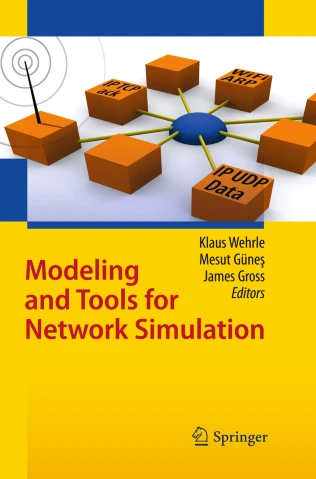
\includegraphics[ width = 1.5cm ]{\pLocalGraphics/978-3-642-12331-3}}}
	\end{overpic}}
\end{frame}

%\begin{frame}\frametitle{Stathopoulos: Personal Web Page \quad {\scriptsize{\mg{\cite{Stathopoulos}}} \,|\, \faUnlock}}
%\center
%	\href{https://www.cs.wm.edu/~andreas/umsa/lectures/cs-sim-pdes.pdf}{
%	\begin{overpic}[ scale = 0.325]
%		{\pLocalGraphics tombstones/Stathopoulos}
%		%\put(2,105) {\color{blue}{https://www.satobs.org/seesat/Aug-2010/0037.html}}
%	\end{overpic}}
%\end{frame}

%\begin{frame}\frametitle{Stathopoulos: Personal Web Page \quad {\scriptsize \raisebox{0.5ex}{\cite{Stathopoulos}} \, \tikz[baseline=-0.5ex]{\draw[thin] (0,0) -- (0,1.0em);} \, \raisebox{0.5ex}{\faUnlock}}}

%     %     %     %     %     %     %     %     %
\subsection{Tools for PDES}
\begin{frame}\frametitle{Experiment}
	I am slide
\end{frame}

\endinput  %  ==  ==  ==  ==  ==  ==  ==  ==  ==


\begin{frame}[allowframebreaks]
    \frametitle{Bibliography}
    \nocite{*}
    \printbibliography
\end{frame}

\end{document}
